\renewcommand{\chaptername}{BAB}
%-----------------------------------------------------------------------------%
\chapter{METODOLOGI PENELITIAN}
%-----------------------------------------------------------------------------%
\vspace{4.5pt}
\setlength{\parskip}{0.5em}
\section{Rancangan Penelitian}\label{sec:rancangan_penelitian}
Tipe Penelitian yang peneliti gunakan disini merupakan penelitian terapan
langsung. Peneliti melakukan \textit{development} secara langsung terhadap Argo
CD yang akan digunakan pada sistem bare-metal (\textit{non-cloud}) yang akan
dikemengembangkan fitur continous deployment dengan ArgoCD

\begin{figure}[h]
  \centering
  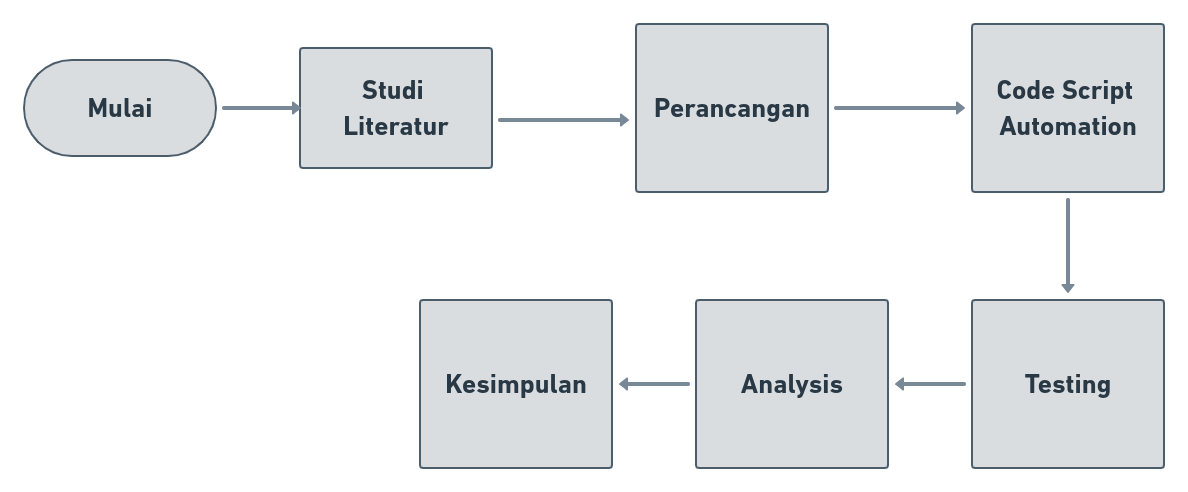
\includegraphics[width=1\textwidth]{figures/Tahapan Skripsi.png}
  \caption{Rancangan Penelitian}
\end{figure}

\subsection{Studi Literatur}\label{subsec:studi_literatur}
Pada tahap studi literatur, peneliti mengumpulkan teori-teori, konsep, dan
temuan penelitian terdahulu yang relevan sebagai landasan dalam melakukan
pengembangan dan implementasi automasi deployment menggunakan Argo CD pada
lingkungan Kubernetes. Studi literatur ini dilakukan dengan menelaah berbagai
sumber seperti buku, jurnal nasional dan internasional, serta dokumentasi resmi
terkait GitOps dan Argo CD.

Peneliti mempelajari konsep dasar GitOps yang menekankan penggunaan repository
Git sebagai sumber kebenaran (single source of truth) untuk seluruh konfigurasi
dan deployment aplikasi \cite{Weaveworks2017}. Selain itu, peneliti juga
mengkaji dokumentasi resmi Argo CD yang menjelaskan fitur, arsitektur, serta
best practice dalam penerapannya pada workflow CI/CD \cite{ArgoCDDocs}.
Penelitian terdahulu dari Korhonen \cite{Korhonen2021} menjadi salah satu
referensi utama, di mana dijelaskan penerapan Argo CD untuk meningkatkan
konsistensi, efisiensi, dan auditability proses deployment aplikasi pada
Kubernetes.

Selain itu, peneliti juga menelaah studi komparatif antara Argo CD dan tools
GitOps lain seperti Flux yang dilakukan oleh Sharma et al. \cite{Sharma2022},
serta kajian terkait tantangan keamanan dalam implementasi Argo CD yang dibahas
oleh Kumar \cite{Kumar2023}. Dengan mengkaji berbagai referensi tersebut,
peneliti memperoleh pemahaman yang komprehensif mengenai teori dan praktik
automasi deployment berbasis GitOps, sehingga dapat merancang dan
mengimplementasikan solusi yang sesuai dengan kebutuhan penelitian.

\subsection{Perancangan (Design)}
Setelah melakukan tahap studi literatur dan analisis kebutuhan sistem, tahap
selanjutnya adalah melakukan perancangan sistem automasi deployment yang akan
diimplementasikan. Pada tahap studi literatur yang telah dilakukan, peneliti
mengambil rancangan dasar dari penelitian-penelitian terdahulu, khususnya model
GitOps yang dibahas oleh Ramadoni \cite{Ramadoni2021} dan arsitektur Argo CD
yang dijelaskan oleh Korhonen \cite{Korhonen2021}.

Pada tahap ini, peneliti melakukan modifikasi terhadap rancangan yang sudah ada
untuk mengadaptasi implementasi Argo CD pada lingkungan bare-metal (non-cloud)
dengan memanfaatkan platform virtualisasi Proxmox. Modifikasi ini penting
dilakukan karena sebagian besar implementasi GitOps dan Argo CD yang ada di
literatur berfokus pada lingkungan cloud \cite{Bolscher2019}, sementara
penelitian ini bertujuan untuk mengimplementasikan solusi serupa pada
infrastruktur on-premise. Perancangan yang dilakukan meliputi beberapa aspek
utama, yaitu:

\begin{enumerate}
  \item Perancangan arsitektur sistem automasi deployment menggunakan Argo CD pada
        lingkungan Kubernetes yang berjalan di atas Proxmox
  \item Perancangan alur kerja sistem sesuai dengan pendekatan pull-based deployment
        yang merupakan karakteristik utama dari GitOps \cite{Weaveworks2017}
  \item Perancangan mekanisme continuous integration yang terintegrasi dengan Argo CD
        untuk membentuk pipeline CI/CD yang lengkap
  \item Perancangan strategi deployment yang efektif untuk aplikasi berbasis
        microservice
\end{enumerate}

\subsection{Implementasi Code Automasi (Coding)}
Tahap implementasi melibatkan pengembangan beberapa komponen kunci yang akan
menjadi fondasi sistem. Implementasi dilakukan dengan bahasa pemrograman Go
untuk microservices dan YAML untuk konfigurasi Kubernetes. Berikut adalah
rincian implementasi yang dilakukan:

\begin{enumerate}[label=\alph*.]
  \item \textbf{Pengembangan Microservices}
        \begin{itemize}
          \item \textbf{Auth Service}: Mengimplementasikan autentikasi berbasis JWT dengan endpoint untuk login dan validasi token
          \item \textbf{Color Service}: Menyediakan API untuk menghasilkan warna acak
          \item \textbf{Prime Generator Service}: Mengimplementasikan algoritma generasi bilangan prima dengan optimasi Sieve of Eratosthenes
          \item \textbf{UI Service}: Dibangun dengan HTMX untuk interaktivitas, bertanggung jawab menampilkan antarmuka pengguna
        \end{itemize}

  \item \textbf{Infrastruktur Kubernetes}
        \begin{itemize}
          \item Konfigurasi manifest Kubernetes untuk setiap komponen
          \item Pembuatan Namespace, Deployment, Service, dan Ingress
          \item Konfigurasi RBAC (Role-Based Access Control) untuk keamanan
          \item Setup Network Policies untuk mengontrol komunikasi antar servis
        \end{itemize}

  \item \textbf{CI/CD Pipeline}
        \begin{itemize}
          \item Implementasi GitHub Actions untuk otomatisasi build dan push image
          \item Konfigurasi ArgoCD untuk continuous deployment
          \item Setup Cloudflare Tunnel untuk akses aman ke cluster
        \end{itemize}
\end{enumerate}

Setiap komponen diimplementasikan dengan mempertimbangkan prinsip-prinsip cloud
native seperti stateless design, horizontal scalability, dan loose coupling.
Kode sumber dikelola dalam repository Git terpusat dengan struktur yang
terorganisir untuk memudahkan kolaborasi dan maintenance. Implementasi ini
menghasilkan arsitektur yang siap di-deploy ke lingkungan Kubernetes yang telah
disiapkan.

\subsection{Pengujian dan Analisis (Testing dan Analysis)}
Dalam pengujian dan analisis hasil dari implementasi yang dibuat akan dilakukan
tahap pengujian terlebih dahulu. Pengujian dan analisis dilakukan untuk mencari
dan mengidentifikasi kesalahan pada sebuah sistem. Pengujian dilakukan dengan
pendekatan sebagai berikut:

\begin{enumerate}[label=\alph*.]
  \item \textbf{Unit Testing}\newline
        Dilakukan pada setiap komponen microservice untuk memastikan setiap fungsi bekerja sesuai harapan. Pengujian mencakup:
        \begin{itemize}
          \item Pengujian fungsi autentikasi pada Auth Service
          \item Pengujian logika generasi bilangan prima pada Prime Generator Service
          \item Pengujian fungsi pengacak warna pada Color Service
        \end{itemize}

  \item \textbf{Integration Testing}\newline
        Pengujian interaksi antar komponen dalam sistem:
        \begin{itemize}
          \item Komunikasi antara UI Service dengan Auth Service untuk proses login
          \item Interaksi antara UI Service dengan Color Service untuk menampilkan warna acak
          \item Integrasi UI Service dengan Prime Generator Service untuk menampilkan bilangan
                prima
        \end{itemize}

  \item \textbf{Black-box Testing}\newline
        Pengujian fungsionalitas sistem secara keseluruhan dari perspektif pengguna akhir:
        \begin{itemize}
          \item Pengujian alur login/logout
          \item Verifikasi tampilan halaman utama
          \item Pengujian fitur generate bilangan prima
          \item Pengujian tampilan warna acak
        \end{itemize}

  \item \textbf{Continuous Deployment Testing}\newline
        Pengujian alur deployment otomatis menggunakan ArgoCD:
        \begin{itemize}
          \item Verifikasi sinkronisasi otomatis antara repository Git dengan cluster
                Kubernetes
          \item Pengujian rollback otomatis saat terjadi kegagalan deployment
          \item Validasi health check dan readiness probe pada setiap service
        \end{itemize}
\end{enumerate}

Setiap temuan dari pengujian didokumentasikan dan dianalisis untuk perbaikan
lebih lanjut. Kriteria keberhasilan pengujian diukur berdasarkan persentase
test case yang berhasil dilalui dan umpan balik dari pengguna akhir.

\subsection{Kesimpulan}
Penyajian kesimpulan merupakan babak final dari keseluruhan proses penelitian.
Pada tahap krusial ini, fokus tidak lagi hanya pada pemaparan data, melainkan
pada sintesis dan interpretasi untuk menarik makna yang lebih dalam dari
seluruh temuan. Seluruh hasil analisis dan evaluasi yang telah dilakukan
dirangkai untuk menjawab rumusan masalah yang menjadi inti dari penelitian ini.
Dengan demikian, bagian ini merumuskan kontribusi utama dari penelitian,
menegaskan implikasi teoretis maupun praktisnya, serta menyajikan rekomendasi
strategis sebagai landasan bagi implementasi atau pengembangan riset di masa
mendatang. \newpage
